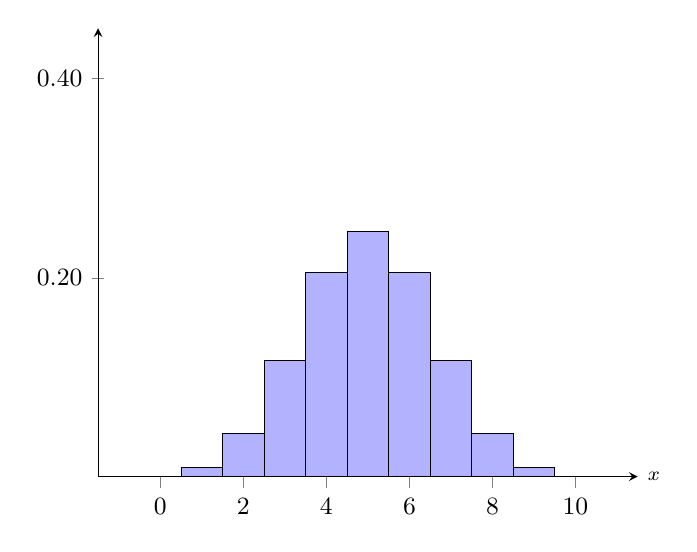
\begin{tikzpicture}[
    declare function={binom(\k,\n,\p)=\n!/(\k!*(\n-\k)!)*\p^\k*(1-\p)^(\n-\k);}
  ]
  \begin{axis}[
      axis lines=left,
      no markers,
      xmin = -1.5, xmax=11.5, ymax=0.45,
      samples at={0,...,10},  
      xtick={0,2,4,6,8,10},
      ytick={0.2,0.4},
      y tick label style={
        /pgf/number format/.cd,
        fixed,
        fixed zerofill,
        precision=2,
        /tikz/.cd
      },
      ticklabel style={font=\small},
      enlargelimits=false,
      clip=false,
      axis on top,
      grid = none,
      ybar=0pt, 
      bar width=1
    ]
    \addplot [fill=blue!30] {binom(x,10,0.5)};
    \node [right] at (axis description cs: 1,0) {\scriptsize $x$};
  \end{axis}
\end{tikzpicture}
